%% ------------- Document Class -------------
%% Original requested class option included 12pt. The local Tectonic cache used
%% for verification does not contain size12.clo or the 12pt Latin Modern fonts
%% and cannot fetch them without network access, so this verified source uses the
%% cached default article size.
\documentclass[letterpaper, final, onecolumn, titlepage]{article}

%% ------------- Mathematics -------------
\usepackage{amsmath}
\usepackage{amssymb}

%% ------------- Page Geometry and Encoding -------------
\usepackage[margin=1in]{geometry}

%% ------------- Paragraph Formatting -------------
\usepackage[shortlabels]{enumitem}

%% ------------- Graphics and Figures -------------
\usepackage{graphicx}

%% ------------- Code Listings -------------
\usepackage{listings}

%% ------------- Section Titles and Spacing -------------

%% ------------- Tables and Colors -------------
\usepackage{booktabs}
\usepackage{longtable}
\usepackage{array}
\usepackage{tabularx}
\usepackage{xcolor}

%% ------------- TikZ and Engineering Diagrams -------------
\usepackage{tikz}
\usetikzlibrary{arrows.meta}

\usepackage[
    colorlinks=true,
    linkcolor=blue,
    urlcolor=blue,
    citecolor=blue
]{hyperref}

\newcommand{\cref}[1]{\ref{#1}}
\newcommand{\Cref}[1]{\ref{#1}}

%% -----------------------------------------------------------------------------
%% Preamble note
%% -----------------------------------------------------------------------------
%% This file keeps the structure and package intent of the requested preamble, but
%% removes duplicate package loads and package-internal amsmath redefinitions that
%% are not valid inside a standalone article document.

%% ------------- Custom math and notation helpers -------------
\providecommand\given{}
\newcommand\SetSymbol[1][]{%
\nonscript\:#1\vert
\allowbreak
\nonscript\:
\mathopen{}}

\newcommand{\bbV}{{\mathbb V}}
\newcommand{\bbR}{{\mathbb R}}

\DeclareRobustCommand{\sig}[1]{\nolinkurl{#1}}
\DeclareRobustCommand{\cfg}[1]{\nolinkurl{#1}}
\DeclareRobustCommand{\view}[1]{\nolinkurl{#1}}
\DeclareRobustCommand{\rtlfile}[1]{\nolinkurl{#1}}
\newcommand{\logiczero}{\ensuremath{1'b0}}
\newcommand{\logicone}{\ensuremath{1'b1}}
\newcommand{\px}{\ensuremath{\mathrm{px}}}
\newcommand{\todoimpl}[1]{\textcolor{BrickRed}{\textbf{Implementation placeholder:} #1}}

\newcolumntype{L}[1]{>{\raggedright\arraybackslash}p{#1}}
\newcolumntype{Y}{>{\raggedright\arraybackslash}X}

%% ------------- Code Listing Style Customization -------------
\definecolor{dkgreen}{rgb}{0,0.4,0}
\definecolor{mauve}{rgb}{0.58,0,0.82}
\definecolor{RoyalBlue}{rgb}{0.10,0.28,0.75}
\definecolor{BrickRed}{rgb}{0.70,0.13,0.13}
\definecolor{Orange}{rgb}{0.95,0.45,0.05}
\definecolor{codeblue}{rgb}{0,0,0.75}
\definecolor{codegreen}{rgb}{0,0.4,0}
\definecolor{codegray}{rgb}{0.5,0.5,0.5}
\definecolor{codepurple}{rgb}{0.58,0,0.82}
\definecolor{backcolour}{rgb}{0.92,0.92,0.92}
\definecolor{headercolor}{HTML}{D9EAD3}
\definecolor{rowtitlecolor}{HTML}{F4CCCC}
\definecolor{lightgraytext}{rgb}{0.45,0.45,0.45}
\definecolor{blueEg}{rgb}{0.25,0.25,0.875}
\definecolor{greenIe}{rgb}{0.15625,0.625,0.15625}
\definecolor{hudcyan}{HTML}{00A6D6}
\definecolor{hudgreen}{HTML}{2CA25F}
\definecolor{hudyellow}{HTML}{D9A441}
\definecolor{hudred}{HTML}{C74343}
\definecolor{hudviolet}{HTML}{8E44AD}
\definecolor{hudslate}{HTML}{34495E}
\definecolor{hudink}{HTML}{111820}

\newcommand{\light}[1]{{\color{lightgraytext}#1}}
\newcommand{\blueExample}[1]{{\color{blueEg}#1}}
\newcommand{\greenExample}[1]{{\color{greenIe}#1}}

\lstdefinestyle{mystyle}{
    backgroundcolor=\color{backcolour},
    commentstyle=\color{codegreen},
    keywordstyle=\color{codeblue},
    numberstyle=\tiny\color{codegray},
    stringstyle=\color{codepurple},
    basicstyle=\footnotesize,
    breakatwhitespace=false,
    breaklines=true,
    captionpos=b,
    keepspaces=true,
    numbers=left,
    numbersep=5pt,
    showspaces=false,
    showstringspaces=false,
    showtabs=false,
    tabsize=2
}
\lstset{style=mystyle}

%% ------------- URL and Paragraph Formatting -------------
\urlstyle{same}
\setlength{\parindent}{10pt}
\setlength{\parskip}{0.75em}
\setcounter{tocdepth}{3}

%% The restricted local Tectonic cache lacks 9pt/8pt Computer Modern metrics.
%% Keep smaller semantic commands available, but map them to the cached 10pt size
%% so verification can run without network package/font fetches.
\makeatletter
\renewcommand\small{\@setfontsize\small{10}{12}}
\renewcommand\footnotesize{\@setfontsize\footnotesize{10}{12}}
\renewcommand\scriptsize{\@setfontsize\scriptsize{10}{12}}
\makeatother

%% ------------- TikZ styles -------------
\tikzset{
  block/.style={draw, rounded corners=2pt, align=center, minimum height=9mm, fill=white, line width=0.45pt},
  smallblock/.style={block, font=\scriptsize, minimum height=7mm},
  bus/.style={-Latex, line width=0.7pt},
  ctrl/.style={-Latex, line width=0.55pt, dashed},
  stage/.style={draw, rounded corners=2pt, fill=RoyalBlue!8, align=center, minimum height=9mm},
  clockdom/.style={draw, dashed, rounded corners=2pt, inner sep=5pt, fill=gray!5},
  screenRegion/.style={draw=hudink, line width=0.45pt, align=center, font=\scriptsize},
  state/.style={draw, circle, minimum size=20mm, align=center, fill=RoyalBlue!7, line width=0.5pt},
  note/.style={draw, rounded corners=2pt, fill=yellow!12, align=left, font=\footnotesize}
}

\title{\textbf{HDMI Rendering Configuration and Control System}\\
\large Source-Aligned Engineering Documentation for the CaelumFusion Flight Visualization Path}
\author{CaelumFusion Flight Control Project}
\date{Revision Draft: 2026-07-05}

\begin{document}
\begin{titlepage}
\thispagestyle{plain}
\maketitle
\vfill
\begin{center}
\begin{tabular}{ll}
\toprule
Document role & Rendering configuration, view selection, and HDMI output reference \\
Implementation baseline & \sig{caelumfusion_top_vga} visualization path \\
Primary pixel format & \sig{vga_rgb[11:0]} with registered \sig{vga_hsync}/\sig{vga_vsync} \\
Nominal active region & 640 by 480 pixels at approximately 60 Hz \\
Clock domains & SYS domain and PIX domain \\
\bottomrule
\end{tabular}
\end{center}
\vfill
\end{titlepage}

\tableofcontents
\listoffigures
\listoftables
\clearpage

\section{Document Scope}

This document defines a rigorous engineering reference for the rendering
configuration and control system that drives the CaelumFusion flight display.
The emphasis is on how configuration fields, control inputs, selected views,
layout choices, and routing decisions determine the final HDMI-visible image.

The checked RTL exposes VGA-style parallel video outputs:
\sig{vga_hsync}, \sig{vga_vsync}, and \sig{vga_rgb[11:0]}. Therefore, this
document uses the term ``HDMI output'' for the downstream visible display
stream after any board-level VGA-to-HDMI bridge, TMDS encoder, or external video
adapter consumes these RGB/sync signals. If a native HDMI encoder is later added,
the contracts in this document should be mapped directly onto the encoder input
signals, for example \sig{hdmi_rgb}, \sig{hdmi_hsync}, \sig{hdmi_vsync}, and
\sig{hdmi_de}.

\subsection{Source Artifacts Reviewed}

The descriptions below are aligned to the following implementation artifacts:

\begin{itemize}[leftmargin=*]
  \item \rtlfile{CaelumFusion_Flight_Control.srcs/sources_1/new/caelumfusion_top_vga.v}
  \item \rtlfile{CaelumFusion_Flight_Control.srcs/sources_1/new/flight_viz_suite_top.v}
  \item \rtlfile{CaelumFusion_Flight_Control.srcs/sources_1/new/flight_visualizer_pix.v}
  \item \rtlfile{CaelumFusion_Flight_Control.srcs/sources_1/new/flight_viz_telemetry_compositor.v}
  \item \rtlfile{CaelumFusion_Flight_Control.srcs/sources_1/new/planar_compass_truth_page_vga.v}
  \item \rtlfile{CaelumFusion_Flight_Control.srcs/sources_1/new/flight_viz_bundle_defs.vh}
  \item \rtlfile{CaelumFusion_Flight_Control.srcs/sources_1/new/vga_timing_640x480_60.v}
\end{itemize}

\subsection{Engineering Assumptions}

\begin{enumerate}[leftmargin=*]
  \item The current top-level output is a VGA-compatible pixel stream. HDMI
  behavior is defined at the level of visible pixels, sync timing, active-video
  gating, and output routing.
  \item The normal flight HUD and the planar compass truth page share the same
  timing envelope and output sync. The truth page replaces RGB data when active.
  \item View-selection features that do not exist as named RTL registers are
  documented as recommended, backward-compatible extension points rather than as
  current implementation facts.
  \item Configuration and control are treated separately: configuration selects
  permitted modes and defaults; control inputs request transitions; registered
  state determines which view is actually displayed.
\end{enumerate}

\section{Rendering Configuration Overview}

\subsection{Purpose}

The rendering configuration system controls how semantic flight data becomes a
deterministic video frame. It is responsible for four engineering contracts:

\begin{enumerate}[leftmargin=*]
  \item \textbf{Representation:} define which raw, derived, authority, navigation,
  wind, metadata, and diagnostic signals are available to the renderer.
  \item \textbf{Timing:} define the active pixel region, blanking intervals, sync
  polarity, reset behavior, and frame boundary used by the output stream.
  \item \textbf{Selection:} define which logical view is selected by operator
  input, build-time defaults, self-test controls, or direct register writes.
  \item \textbf{Routing:} define which rendered RGB source reaches the HDMI-visible
  output after layer priority, full-page replacement, and active-video gating.
\end{enumerate}

\subsection{Implemented Pipeline}

\Cref{fig:pipeline} shows the current source-aligned rendering pipeline. The
SYS-domain sensor and derived-state records are normalized into the canonical
visualization bundle, crossed into the pixel domain through an explicit CDC
snapshot path, rendered as a normal flight HUD, and optionally replaced by the
planar compass truth page.

\begin{figure}[htbp]
\centering
\begin{tikzpicture}[font=\scriptsize, scale=0.84, transform shape]
  \node[stage] (sensors) at (0,1.2) {Sensor suites\\BMP, ACC, MAG};
  \node[stage] (derived) at (2.7,1.2) {Derived state\\altitude, speed, roll, heading};
  \node[stage] (authority) at (2.7,-0.2) {Authority gates\\phase, safety, policy};
  \node[stage] (model) at (5.4,1.2) {\sig{flight_viz_model_sys}\\canonical semantic image};
  \node[stage] (cdc) at (8.1,1.2) {\sig{flight_viz_bundle_cdc}\\SYS to PIX snapshot};
  \node[stage] (renderer) at (10.8,1.2) {\sig{flight_visualizer_pix}\\base scene + text overlay};
  \node[stage] (truth) at (13.5,1.2) {\sig{planar_compass_truth_page_vga}\\full-page replacement};
  \node[stage] (hdmi) at (16.2,1.2) {HDMI-visible\\RGB/sync stream};

  \draw[bus] (sensors) -- (derived);
  \draw[bus] (derived) -- (model);
  \draw[bus] (authority) -| (model);
  \draw[bus] (model) -- node[above, font=\scriptsize]{800-bit bundle} (cdc);
  \draw[bus] (cdc) -- node[above, font=\scriptsize]{shadow + pulse} (renderer);
  \draw[bus] (renderer) -- node[above, font=\scriptsize]{\sig{viz_vga_*}} (truth);
  \draw[bus] (truth) -- node[above, font=\scriptsize]{\sig{vga_*}} (hdmi);

  \draw[clockdom] (-1.1,-1.0) rectangle (6.5,2.1);
  \node[font=\scriptsize] at (2.7,2.35) {SYS domain};
  \draw[clockdom] (7.1,-1.0) rectangle (14.6,2.1);
  \node[font=\scriptsize] at (10.8,2.35) {PIX domain};
\end{tikzpicture}
\caption{Source-aligned rendering-to-HDMI pipeline. The current implementation
uses VGA signal names, but the routing and visible-pixel contract are directly
applicable to a downstream HDMI bridge or encoder.}
\label{fig:pipeline}
\end{figure}

\subsection{Configuration Field Model}

\Cref{tab:config-fields} defines a consolidated configuration model. Fields
marked ``implemented'' are present in the inspected RTL. Fields marked
``extension'' are recommended placeholders for future control registers or build
parameters.

\begin{longtable}{L{0.21\textwidth} L{0.24\textwidth} L{0.16\textwidth} L{0.30\textwidth}}
\caption{Rendering configuration fields and their HDMI-visible effects.}
\label{tab:config-fields}\\
\toprule
Configuration field & Implementation name & Status & HDMI-visible effect \\
\midrule
\endfirsthead
\toprule
Configuration field & Implementation name & Status & HDMI-visible effect \\
\midrule
\endhead
Active width and height &
\sig{H_ACTIVE}, \sig{V_ACTIVE} &
Implemented &
Defines the visible raster. Current default is 640 by 480 pixels. Pixels outside this region are treated as inactive video and are blacked by the normal HUD path. \\
\addlinespace
Horizontal and vertical blanking &
\sig{H_FP}, \sig{H_SYNC}, \sig{H_BP}, \sig{V_FP}, \sig{V_SYNC}, \sig{V_BP} &
Implemented &
Defines sync timing and the total raster. The normal HUD and truth page share this timing envelope. \\
\addlinespace
Sync polarity &
\sig{HSYNC_POL}, \sig{VSYNC_POL} &
Implemented &
Determines active level of the sync pulses. The default value 0 corresponds to negative sync in the VGA timing generator. \\
\addlinespace
Build sensor source mode &
\sig{CAELUM_SENSOR_SPI} &
Implemented as compile-time define &
Changes which sensor suite publishes the semantic data that becomes text, validity colors, heading, altitude, and authority evidence. It should not alter pixel timing or region boundaries. \\
\addlinespace
Accelerometer source priority &
\sig{USE_LIS3DH_I2C_ACC}, \sig{USE_ADXL362_SPI_ACC} &
Implemented as parameters &
Changes the source feeding ACC validity and roll-related display regions. Failed or stale ACC data visibly degrades the horizon and vertical-vector regions. \\
\addlinespace
Magnetometer source enable &
\sig{USE_CMPS2_MMC3416_MAG} &
Implemented as parameter &
Selects the CMPS2/MMC3416 heading source for MAG validity, compass, and truth-page diagnostic output. \\
\addlinespace
Truth-page default &
\sig{COMPASS_TRUTH_PAGE_DEFAULT} &
Implemented as parameter &
Forces the planar compass truth page to replace the normal flight HUD RGB stream when nonzero. Sync remains passed through from the normal HUD path. \\
\addlinespace
Momentary page request &
\sig{btn_page_raw}, \sig{page_enable_sys} &
Implemented as board input/control wire &
Requests the truth page. In the current top, the same raw button is also wired to \sig{viz_selftest_en_sys}, so page request and normal-HUD self-test stimulus are coupled. \\
\addlinespace
Visualization self-test &
\sig{viz_selftest_en_sys} &
Implemented &
Substitutes a deterministic self-test semantic image before the visualization model. This changes the normal HUD data content; if the truth page is also active, the self-test HUD is behind the replacement page. \\
\addlinespace
Logical view selection &
\sig{cfg_view_sel[2:0]} &
Extension &
Recommended registered selector for \view{VIEW_FLIGHT_HUD}, \view{VIEW_COMPASS_TRUTH}, \view{VIEW_SELFTEST_HUD}, and future diagnostic pages. \\
\addlinespace
Layout mode &
\sig{cfg_layout_sel[2:0]} &
Extension &
Recommended selector for single-view, split-view, multi-panel, overlay, debug/status, and composite arrangements. Current normal HUD implements a fixed composite layout. \\
\addlinespace
Output route &
\sig{cfg_output_route[1:0]} &
Extension &
Recommended selector for HDMI, mirror, test-pattern, or disabled output paths. Current RTL has one board-facing RGB/sync path. \\
\bottomrule
\end{longtable}

\subsection{Data Representation Contract}

The normal renderer consumes a canonical 800-bit visualization bundle. The bundle
contains raw sensor summary fields, derived-state validity and provenance,
authority policy evidence, navigation and wind evidence, and platform metadata.
The renderer must treat this bundle as a semantic contract, not as arbitrary raw
pixels. The most important classes are summarized in \cref{tab:bundle-classes}.

\begin{table}[htbp]
\centering
\small
\begin{tabularx}{\textwidth}{L{0.22\textwidth} L{0.24\textwidth} Y}
\toprule
Bundle class & Representative fields & Display responsibility \\
\midrule
Raw sensor summaries &
\sig{bmp_valid}, \sig{bmp_status}, \sig{bmp_age_ms}, \sig{acc_*}, \sig{mag_*} &
Top health strip, text overlay, stale/fault color coding, and provenance for derived quantities. \\
\addlinespace
Derived-state quantities &
\sig{der_altitude_cm}, \sig{der_vertical_speed_cms}, \sig{der_roll_mdeg}, \sig{der_heading_mdeg} &
Altitude tape, vertical-speed tape, charts, horizon, roll-plane vector, and compass. \\
\addlinespace
Derived provenance &
\sig{der_bmp_seq_ref}, \sig{der_acc_seq_ref}, \sig{der_mag_seq_ref}, \sig{der_*_fresh} &
Determines whether plotted values are fresh, stale, unavailable, or backed by valid sensor references. \\
\addlinespace
Authority evidence &
\sig{auth_target_cm}, \sig{auth_pred_no_cm}, \sig{auth_pred_full_cm}, \sig{auth_brake_cmd_u8}, \sig{auth_gate_flags} &
Apogee authority ladder, target marker, uncertainty band, command level, phase strip, and actuation gate strip. \\
\addlinespace
Navigation and wind evidence &
\sig{nav_downrange_m}, \sig{nav_crossrange_m}, \sig{wind_x_cms}, \sig{wind_y_cms}, \sig{wind_z_cms} &
Landing dispersion and wind-estimator viewport. The current top drives these unavailable, so the renderer should visibly degrade rather than invent data. \\
\addlinespace
Metadata and counters &
\sig{i2c_nack_count}, \sig{i2c_timeout_count}, \sig{txn_rate_hz}, \sig{cdc_update_count}, \sig{build_id}, \sig{schema_word} &
Bottom debug/status strip and operator confidence metadata. \\
\bottomrule
\end{tabularx}
\caption{Semantic classes in the visualization bundle.}
\label{tab:bundle-classes}
\end{table}

\section{HDMI Output Mapping}

\subsection{Top-Level Routing Rule}

The top-level display route is a two-stage selection:

\begin{enumerate}[leftmargin=*]
  \item \sig{flight_visualizer_pix} always generates the normal flight HUD stream
  \sig{viz_vga_hsync}, \sig{viz_vga_vsync}, and \sig{viz_vga_rgb}.
  \item \sig{planar_compass_truth_page_vga} passes sync through and either passes
  normal HUD RGB through or replaces it with a full-screen diagnostic page.
\end{enumerate}

The current truth-page active equation is:

\begin{equation}
\mathrm{page\_active}
=
\begin{cases}
1, & C_{\mathrm{truth\_default}} \ne 0, \\
\mathrm{page\_enable\_pix}, & C_{\mathrm{truth\_default}} = 0.
\end{cases}
\label{eq:page-active}
\end{equation}

The final top-level RGB route is:

\begin{equation}
\mathrm{RGB}_{out}
=
\begin{cases}
\mathrm{RGB}_{truth}, & \mathrm{page\_active}=1,\\
\mathrm{RGB}_{flight}, & \mathrm{page\_active}=0.
\end{cases}
\label{eq:top-rgb-route}
\end{equation}

The final top-level sync route is:

\begin{equation}
\mathrm{HSYNC}_{out}=\mathrm{HSYNC}_{flight},
\qquad
\mathrm{VSYNC}_{out}=\mathrm{VSYNC}_{flight}.
\label{eq:sync-pass}
\end{equation}

\subsection{Current Configuration-to-Output Table}

\begin{table}[htbp]
\centering
\small
\begin{tabularx}{\textwidth}{L{0.18\textwidth} L{0.16\textwidth} L{0.20\textwidth} Y}
\toprule
\sig{COMPASS_TRUTH_PAGE_DEFAULT} & \sig{btn_page_raw} & Selected HDMI-visible view & Notes \\
\midrule
0 & 0 & Normal flight HUD & Flight display uses real semantic data unless another upstream source option changes the data. \\
0 & 1 & Planar compass truth page & The same button also enables \sig{viz_selftest_en_sys} in the current top, so the normal HUD behind the truth page receives self-test data. \\
1 & 0 & Planar compass truth page & Page is forced active by parameter. Normal HUD still exists upstream but is not visible. \\
1 & 1 & Planar compass truth page & Page remains active. Self-test semantic stimulus is also enabled for the upstream normal HUD. \\
\bottomrule
\end{tabularx}
\caption{Current top-level output mapping from truth-page controls to HDMI-visible output.}
\label{tab:current-output-map}
\end{table}

\subsection{Normal Flight HUD Layer Priority}

Within the normal flight HUD, layer priority is deterministic and registered in
one render-aligned output stage. Text overlay has priority above the base scene,
and inactive pixels are black:

\begin{equation}
\mathrm{RGB}_{flight}
=
\begin{cases}
0, & \mathrm{render\_active\_q}=0,\\
\mathrm{RGB}_{text}, & \mathrm{render\_active\_q}=1 \land \mathrm{render\_overlay\_on\_q}=1,\\
\mathrm{RGB}_{base}, & \mathrm{render\_active\_q}=1 \land \mathrm{render\_overlay\_on\_q}=0.
\end{cases}
\label{eq:flight-layer-priority}
\end{equation}

\begin{table}[htbp]
\centering
\small
\begin{tabularx}{\textwidth}{L{0.20\textwidth} L{0.24\textwidth} Y}
\toprule
Priority & Condition & HDMI-visible result \\
\midrule
Highest & \sig{page_active} asserted in truth-page module & Full-screen planar compass diagnostic RGB replaces the normal HUD RGB. \\
High & Normal HUD active and \sig{render_overlay_on_q} asserted & Telemetry text RGB is displayed at the selected glyph pixel. \\
Medium & Normal HUD active and no text overlay pixel selected & Base instrument scene RGB is displayed. \\
Lowest & Normal HUD inactive video & RGB is black regardless of base or text state. \\
\bottomrule
\end{tabularx}
\caption{Effective layer priority from full-page routing down to inactive-video blacking.}
\label{tab:layer-priority}
\end{table}

\subsection{Timing and Active-Video Mapping}

The timing generator defines a 640 by 480 visible window inside an 800 by 525
nominal raster:

\begin{align}
H_{total} &= H_{active}+H_{fp}+H_{sync}+H_{bp},\\
V_{total} &= V_{active}+V_{fp}+V_{sync}+V_{bp}.
\end{align}

With the current defaults:

\begin{equation}
H_{total}=640+16+96+48=800,
\qquad
V_{total}=480+10+2+33=525.
\end{equation}

The normal HUD considers the current pixel visible only when:

\begin{equation}
\mathrm{active} = (x < H_{active}) \land (y < V_{active}).
\label{eq:active-video}
\end{equation}

\section{HDMI View Selection Logic}

\subsection{Control Input, Selection State, and Rendered Output}

A robust view-selection design must not conflate an operator control pulse with
the selected view or with the rendered pixels. \Cref{tab:control-state-output}
defines the distinction used throughout this document.

\begin{table}[htbp]
\centering
\small
\begin{tabularx}{\textwidth}{L{0.22\textwidth} L{0.25\textwidth} Y}
\toprule
Concept & Examples & Contract \\
\midrule
Control input & \sig{btn_page_raw}, \sig{view_next_pulse}, \sig{view_prev_pulse}, \sig{view_direct_valid} & May be asynchronous or momentary. Must be synchronized or debounced before it updates registered selection state. \\
\addlinespace
Selection state & \sig{view_sel_q}, \sig{page_active}, \sig{COMPASS_TRUTH_PAGE_DEFAULT} & Stable state that determines which logical view is selected for a frame or longer. \\
\addlinespace
Rendered output & \sig{vga_rgb}, \sig{vga_hsync}, \sig{vga_vsync}, future \sig{hdmi_*} & Physical video stream after routing, layer priority, blanking, and output-format conversion. \\
\bottomrule
\end{tabularx}
\caption{Control input, selection state, and rendered HDMI output are separate contracts.}
\label{tab:control-state-output}
\end{table}

\subsection{Current Implemented View Selection}

The current top-level design implements a two-output-view selection:

\begin{itemize}[leftmargin=*]
  \item \view{VIEW_FLIGHT_HUD}: normal three-column flight display with top
  health strip, text overlay, charts, authority ladder, and primary instruments.
  \item \view{VIEW_COMPASS_TRUTH}: full-screen planar compass truth page that
  replaces normal HUD RGB while preserving normal HUD sync.
\end{itemize}

The current implementation does not expose next/previous view controls, direct
view register writes, or a multi-state view selector register. Those controls
are recommended as the backward-compatible extension shown in
\cref{fig:view-state-machine}.

\subsection{Recommended View Selector State Machine}

\begin{figure}[htbp]
\centering
\begin{tikzpicture}[font=\small]
  \node[state] (flight) at (0,2.2) {\view{VIEW_FLIGHT}\\HUD};
  \node[state] (truth) at (4.8,2.2) {\view{VIEW_COMPASS}\\TRUTH};
  \node[state] (selftest) at (0,0) {\view{VIEW_SELFTEST}\\HUD};
  \node[state] (reserved) at (4.8,0) {\view{RESERVED}\\hold/default};

  \draw[bus] (flight) to[bend left=16] node[above, font=\scriptsize]{next/direct} (truth);
  \draw[bus] (truth) to[bend left=16] node[below, font=\scriptsize]{prev/direct} (flight);
  \draw[bus] (flight) to[bend right=14] node[left, font=\scriptsize]{direct self-test} (selftest);
  \draw[bus] (selftest) to[bend right=14] node[right, font=\scriptsize]{reset/direct flight} (flight);
  \draw[bus] (truth) -- node[right, font=\scriptsize]{invalid direct} (reserved);
  \draw[bus] (reserved) -- node[below, font=\scriptsize]{reset/default} (selftest);

  \draw[ctrl] (flight.north) .. controls (-0.9,3.25) and (0.9,3.25) .. node[above, font=\scriptsize]{hold} (flight.north);
  \draw[ctrl] (truth.north) .. controls (3.9,3.25) and (5.7,3.25) .. node[above, font=\scriptsize]{hold} (truth.north);
\end{tikzpicture}
\caption{Recommended state-machine-style view selector. The current RTL directly
implements the flight HUD and compass truth page paths, while the self-test and
reserved states should be made explicit before adding more page controls.}
\label{fig:view-state-machine}
\end{figure}

\subsection{Recommended Transition Rules}

\begin{table}[htbp]
\centering
\small
\begin{tabularx}{\textwidth}{L{0.18\textwidth} L{0.23\textwidth} L{0.22\textwidth} Y}
\toprule
Event & Condition & Next state & Required output behavior \\
\midrule
Reset/default & \sig{rst} asserted or configuration reload & \view{VIEW_COMPASS_TRUTH} if \sig{COMPASS_TRUTH_PAGE_DEFAULT != 0}; otherwise \view{VIEW_FLIGHT_HUD} & Output state must be deterministic after reset release. \\
\addlinespace
Next view & Debounced \sig{view_next_pulse} & Next valid state in ordered view list & State changes at a controlled boundary; recommended boundary is vertical blank or next frame. \\
\addlinespace
Previous view & Debounced \sig{view_prev_pulse} & Previous valid state in ordered view list & Same frame-boundary update rule as next view. \\
\addlinespace
Direct selection & \sig{view_direct_valid} and legal \sig{view_direct_id} & Requested state & Illegal direct values must not decode into arbitrary mux selects. \\
\addlinespace
Invalid or reserved & Illegal \sig{view_direct_id}, unimplemented state, or parity/check failure & Hold current state or force documented safe default & Recommended behavior is hold-current plus a sticky \sig{cfg_invalid_view} flag. For bring-up, forcing \view{VIEW_FLIGHT_HUD} is also acceptable if documented. \\
\bottomrule
\end{tabularx}
\caption{Recommended view-selection transition rules.}
\label{tab:transition-rules}
\end{table}

\subsection{Reference Selection Pseudocode}

\begin{figure}[htbp]
\centering
\begin{minipage}{0.92\textwidth}
\begin{lstlisting}
// Frame-stable view selector update.
// Inputs are synchronized/debounced before this block.
if (rst) begin
    view_sel_q <= default_view;
end else if (frame_boundary) begin
    if (view_direct_valid && direct_view_is_legal) begin
        view_sel_q <= view_direct_id;
    end else if (view_direct_valid && !direct_view_is_legal) begin
        cfg_invalid_view <= 1'b1;
        view_sel_q <= view_sel_q;       // hold current state
    end else if (view_next_pulse) begin
        view_sel_q <= next_legal_view(view_sel_q);
    end else if (view_prev_pulse) begin
        view_sel_q <= prev_legal_view(view_sel_q);
    end else begin
        view_sel_q <= view_sel_q;       // hold current state
    end
end
\end{lstlisting}
\end{minipage}
\caption{Reference frame-stable view selector pseudocode.}
\label{fig:view-selector-pseudocode}
\end{figure}

\section{HDMI Layout and Arrangement Diagrams}

\subsection{Implemented Normal Flight HUD Layout}

\Cref{fig:normal-layout} shows the implemented normal flight HUD screen layout.
The coordinate ranges are listed in \cref{tab:region-map}. The logical
coordinate origin is the upper-left active pixel. The diagram is drawn in display
orientation rather than mathematical orientation.

\begin{figure}[htbp]
\centering
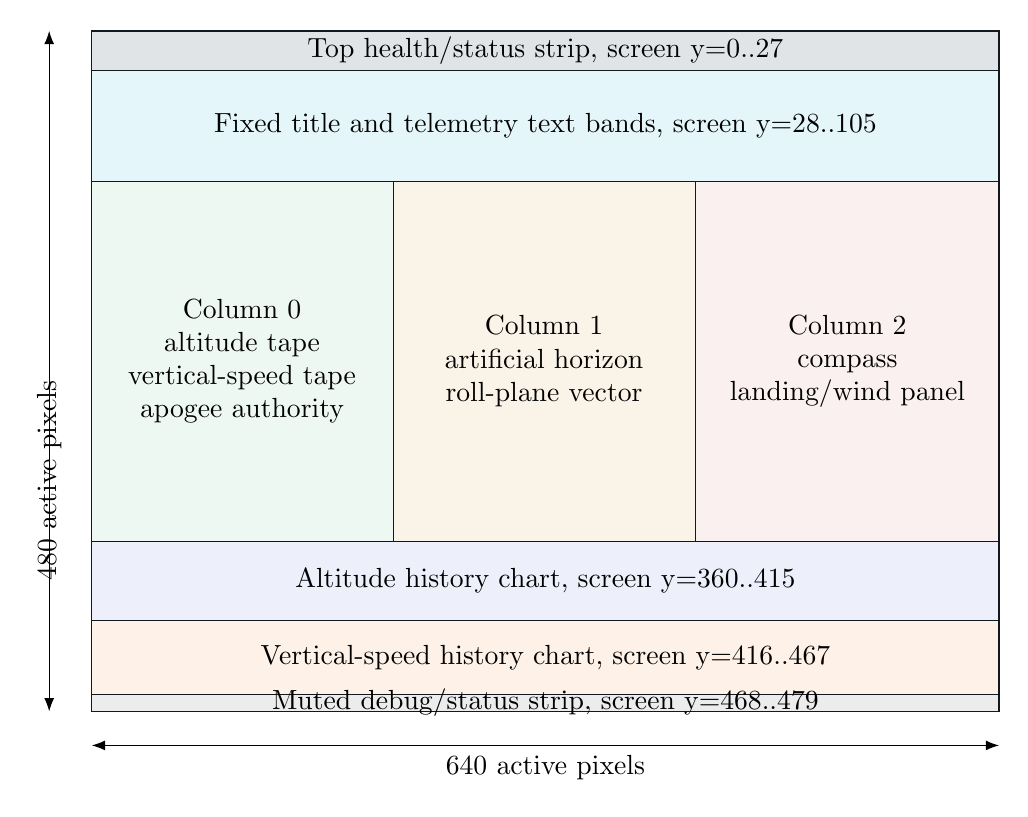
\begin{tikzpicture}[x=0.018cm,y=0.018cm,font=\scriptsize]
  \draw[fill=black!3, draw=hudink] (0,0) rectangle (640,480);

  \draw[screenRegion, fill=hudslate!15] (0,452) rectangle (640,480);
  \node at (320,466) {Top health/status strip, screen y=0..27};

  \draw[screenRegion, fill=hudcyan!10] (0,374) rectangle (640,452);
  \node at (320,413) {Fixed title and telemetry text bands, screen y=28..105};

  \draw[screenRegion, fill=hudgreen!8] (0,120) rectangle (213,374);
  \node[align=center] at (106,247) {Column 0\\altitude tape\\vertical-speed tape\\apogee authority};

  \draw[screenRegion, fill=hudyellow!12] (213,120) rectangle (426,374);
  \node[align=center] at (319,247) {Column 1\\artificial horizon\\roll-plane vector};

  \draw[screenRegion, fill=hudred!8] (426,120) rectangle (640,374);
  \node[align=center] at (533,247) {Column 2\\compass\\landing/wind panel};

  \draw[screenRegion, fill=RoyalBlue!8] (0,64) rectangle (640,120);
  \node at (320,92) {Altitude history chart, screen y=360..415};

  \draw[screenRegion, fill=Orange!10] (0,12) rectangle (640,64);
  \node at (320,38) {Vertical-speed history chart, screen y=416..467};

  \draw[screenRegion, fill=gray!15] (0,0) rectangle (640,12);
  \node at (320,6) {Muted debug/status strip, screen y=468..479};

  \draw[Latex-Latex] (0,-24) -- node[below]{640 active pixels} (640,-24);
  \draw[Latex-Latex] (-30,0) -- node[left, rotate=90]{480 active pixels} (-30,480);
\end{tikzpicture}
\caption{Implemented normal flight HUD arrangement. Screen y ranges increase
downward in RTL, but this diagram is drawn upright for readability.}
\label{fig:normal-layout}
\end{figure}

\begin{table}[htbp]
\centering
\small
\begin{tabularx}{\textwidth}{L{0.23\textwidth} L{0.16\textwidth} L{0.16\textwidth} Y}
\toprule
Region & x range & y range & Primary content \\
\midrule
Top health/status strip & 0..639 & 0..27 & BMP, ACC, MAG health blocks and age bars. \\
Text title and telemetry band & 0..639 & 28..105 & Top strip labels, left/mid/right panel text, and title rows. \\
Column 0 primary instruments & 0..212 & 106..359 & Altitude tape, vertical-speed tape, and apogee authority ladder. \\
Column 1 primary instruments & 213..425 & 106..359 & Artificial horizon and roll-plane vertical vector. \\
Column 2 primary instruments & 426..639 & 106..359 & Compass, landing dispersion, and wind estimator. \\
Altitude chart & 0..639 & 360..415 & History ring plot with newest-sample cursor at right edge. \\
Vertical-speed chart & 0..639 & 416..467 & Signed vertical-speed history with zero line and newest-sample cursor. \\
Bottom debug strip & 0..639 & 468..479 & Compact metadata, counters, schema, and frame/build evidence. \\
\bottomrule
\end{tabularx}
\caption{Normal HUD screen-region map.}
\label{tab:region-map}
\end{table}

\subsection{Logical Layout Mode Vocabulary}

The current implementation is a fixed composite layout. Future configuration
registers should name layout modes explicitly so HDMI behavior is reviewable.
\Cref{fig:layout-vocabulary} defines a recommended vocabulary.

\begin{figure}[htbp]
\centering
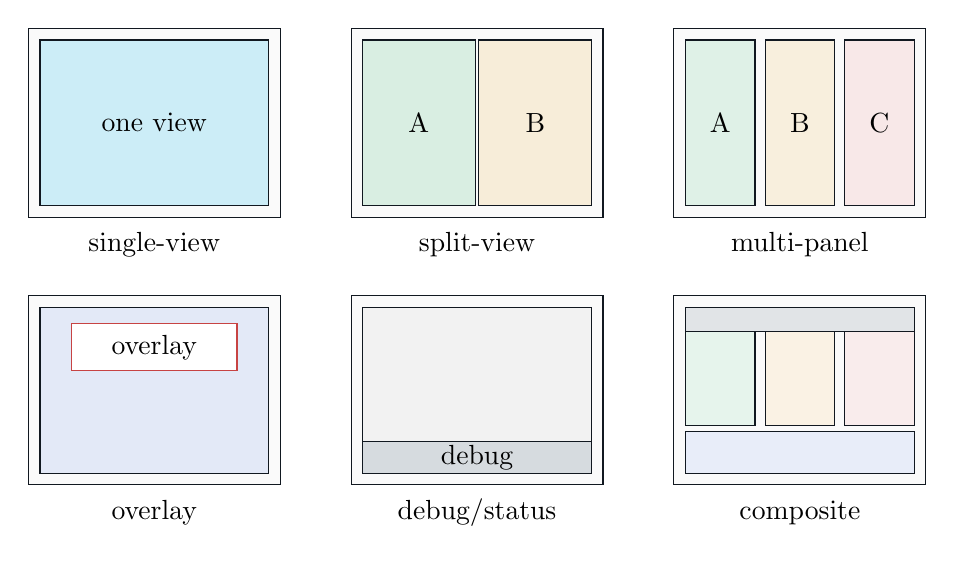
\begin{tikzpicture}[font=\scriptsize]
  \newcommand{\miniscreen}[4]{%
    \begin{scope}[shift={(#1,#2)}]
      \draw[fill=black!2, draw=hudink] (0,0) rectangle (3.2,2.4);
      #4
      \node[align=center] at (1.6,-0.35) {#3};
    \end{scope}}

  \miniscreen{0}{0}{single-view}{
    \draw[fill=hudcyan!20, draw=hudink] (0.15,0.15) rectangle (3.05,2.25);
    \node at (1.6,1.2) {one view};
  }

  \miniscreen{4.1}{0}{split-view}{
    \draw[fill=hudgreen!18, draw=hudink] (0.15,0.15) rectangle (1.58,2.25);
    \draw[fill=hudyellow!20, draw=hudink] (1.62,0.15) rectangle (3.05,2.25);
    \node at (0.86,1.2) {A};
    \node at (2.34,1.2) {B};
  }

  \miniscreen{8.2}{0}{multi-panel}{
    \draw[fill=hudgreen!15, draw=hudink] (0.15,0.15) rectangle (1.03,2.25);
    \draw[fill=hudyellow!18, draw=hudink] (1.16,0.15) rectangle (2.04,2.25);
    \draw[fill=hudred!12, draw=hudink] (2.17,0.15) rectangle (3.05,2.25);
    \node at (0.59,1.2) {A};
    \node at (1.60,1.2) {B};
    \node at (2.61,1.2) {C};
  }

  \miniscreen{0}{-3.4}{overlay}{
    \draw[fill=RoyalBlue!12, draw=hudink] (0.15,0.15) rectangle (3.05,2.25);
    \draw[fill=white, draw=hudred, line width=0.5pt] (0.55,1.45) rectangle (2.65,2.05);
    \node at (1.6,1.75) {overlay};
  }

  \miniscreen{4.1}{-3.4}{debug/status}{
    \draw[fill=gray!10, draw=hudink] (0.15,0.15) rectangle (3.05,2.25);
    \draw[fill=hudslate!20, draw=hudink] (0.15,0.15) rectangle (3.05,0.55);
    \node at (1.6,0.35) {debug};
  }

  \miniscreen{8.2}{-3.4}{composite}{
    \draw[fill=hudslate!15, draw=hudink] (0.15,1.95) rectangle (3.05,2.25);
    \draw[fill=hudgreen!12, draw=hudink] (0.15,0.75) rectangle (1.03,1.95);
    \draw[fill=hudyellow!14, draw=hudink] (1.16,0.75) rectangle (2.04,1.95);
    \draw[fill=hudred!10, draw=hudink] (2.17,0.75) rectangle (3.05,1.95);
    \draw[fill=RoyalBlue!10, draw=hudink] (0.15,0.15) rectangle (3.05,0.68);
  }
\end{tikzpicture}
\caption{Recommended layout-mode vocabulary. The current flight HUD corresponds
to the composite arrangement.}
\label{fig:layout-vocabulary}
\end{figure}

\subsection{Source-to-Region Mapping}

\Cref{fig:source-region-map} maps logical rendering sources to physical HDMI
regions. This is the engineering distinction that prevents raw data, derived
estimates, operator diagnostics, and display formatting from being confused.

\begin{figure}[htbp]
\centering
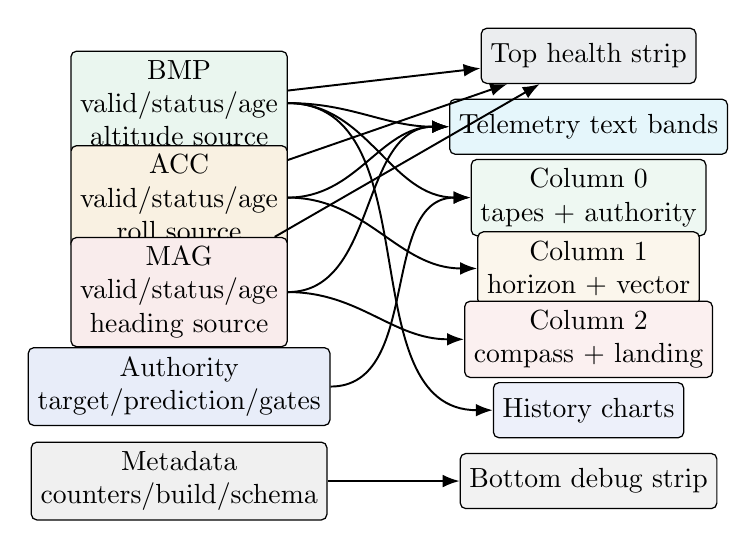
\begin{tikzpicture}[font=\scriptsize]
  \node[smallblock, fill=hudgreen!10] (bmp) at (0,4.8) {BMP\\valid/status/age\\altitude source};
  \node[smallblock, fill=hudyellow!15] (acc) at (0,3.6) {ACC\\valid/status/age\\roll source};
  \node[smallblock, fill=hudred!10] (mag) at (0,2.4) {MAG\\valid/status/age\\heading source};
  \node[smallblock, fill=RoyalBlue!10] (auth) at (0,1.2) {Authority\\target/prediction/gates};
  \node[smallblock, fill=gray!12] (meta) at (0,0) {Metadata\\counters/build/schema};

  \node[smallblock, fill=hudslate!10] (top) at (5.2,5.4) {Top health strip};
  \node[smallblock, fill=hudcyan!10] (text) at (5.2,4.5) {Telemetry text bands};
  \node[smallblock, fill=hudgreen!8] (col0) at (5.2,3.6) {Column 0\\tapes + authority};
  \node[smallblock, fill=hudyellow!10] (col1) at (5.2,2.7) {Column 1\\horizon + vector};
  \node[smallblock, fill=hudred!8] (col2) at (5.2,1.8) {Column 2\\compass + landing};
  \node[smallblock, fill=RoyalBlue!8] (charts) at (5.2,0.9) {History charts};
  \node[smallblock, fill=gray!10] (debug) at (5.2,0) {Bottom debug strip};

  \draw[bus] (bmp) -- (top);
  \draw[bus] (acc) -- (top);
  \draw[bus] (mag) -- (top);
  \draw[bus] (bmp.east) to[out=0,in=180] (text.west);
  \draw[bus] (acc.east) to[out=0,in=180] (text.west);
  \draw[bus] (mag.east) to[out=0,in=180] (text.west);
  \draw[bus] (bmp.east) to[out=0,in=180] (col0.west);
  \draw[bus] (auth.east) to[out=0,in=180] (col0.west);
  \draw[bus] (acc.east) to[out=0,in=180] (col1.west);
  \draw[bus] (mag.east) to[out=0,in=180] (col2.west);
  \draw[bus] (bmp.east) to[out=0,in=180] (charts.west);
  \draw[bus] (meta.east) to[out=0,in=180] (debug.west);
\end{tikzpicture}
\caption{Logical source-to-region mapping for the normal flight HUD.}
\label{fig:source-region-map}
\end{figure}

\section{Frame-Stable Rendering Contract}

\subsection{Bundle Commit Rule}

The PIX renderer does not directly change the committed semantic bundle on an
arbitrary CDC update pulse. Instead, updates are captured into a pending register
and committed on \sig{vsync_edge}. This ensures that the displayed semantic image
does not change mid-frame.

Let $B_p$ be the pending bundle, $B_q$ the committed bundle, and $U$ the update
pulse. At a frame boundary:

\begin{equation}
B_q^{+} =
\begin{cases}
B_{in}, & U=1,\\
B_p, & U=0 \land B_p \text{ valid},\\
B_q, & \text{otherwise}.
\end{cases}
\label{eq:bundle-commit}
\end{equation}

The chart write pointer uses the same pending-and-frame-boundary pattern. This
prevents a new history write pointer from being displayed before the corresponding
history values are coherently visible to the renderer.

\subsection{CDC Publication Rule}

The SYS-domain visualization model produces a semantic key. A publication is
requested when that key changes or when self-test is enabled and its periodic
tick fires:

\begin{equation}
\mathrm{publish\_request}
 =
(\mathrm{viz\_key\_model\_sys} \ne \mathrm{viz\_key\_prev\_sys})
\lor
(\mathrm{viz\_selftest\_en\_sys} \land \mathrm{selftest\_tick\_sys}).
\label{eq:publish-request}
\end{equation}

The CDC contract is snapshot based: source logic holds the bundle, toggles a
publication event, destination logic synchronizes the event, then samples the
held bundle into a PIX-domain shadow register. Any HDMI documentation or future
view-control expansion must preserve this single coherent semantic image
contract.

\section{Configuration and Output Mapping Tables}

\subsection{Logical View Map}

\begin{table}[htbp]
\centering
\small
\begin{tabularx}{\textwidth}{L{0.21\textwidth} L{0.20\textwidth} L{0.22\textwidth} Y}
\toprule
Logical view & Current source & HDMI region coverage & Notes \\
\midrule
\view{VIEW_FLIGHT_HUD} & \sig{flight_visualizer_pix} & Full active frame, internally divided into fixed regions & Implemented normal display. Includes base scene, text overlay, charts, and debug strip. \\
\addlinespace
\view{VIEW_COMPASS_TRUTH} & \sig{planar_compass_truth_page_vga} & Full active frame replacement & Implemented diagnostic page. Replaces RGB only; sync is passed through. \\
\addlinespace
\view{VIEW_SELFTEST_HUD} & \sig{flight_viz_suite_top} with \sig{viz_selftest_en_sys} & Normal flight HUD layout with deterministic synthetic data & Implemented as stimulus mode but not currently exposed as a separate visible view selector. \\
\addlinespace
\view{VIEW_TEST_PATTERN} & \todoimpl{future} & Full active frame or selected region & Recommended for HDMI bring-up and monitor compatibility testing. \\
\addlinespace
\view{VIEW_RESERVED} & \todoimpl{future} & No arbitrary decode & Reserved values must hold current output or force a documented safe default. \\
\bottomrule
\end{tabularx}
\caption{Logical HDMI view map.}
\label{tab:logical-view-map}
\end{table}

\subsection{Output Format Map}

\begin{table}[htbp]
\centering
\small
\begin{tabularx}{\textwidth}{L{0.20\textwidth} L{0.20\textwidth} Y}
\toprule
Signal or format item & Current RTL representation & HDMI interpretation \\
\midrule
Pixel data & \sig{vga_rgb[11:0]} & Packed RGB444. A downstream HDMI bridge may expand to RGB888 by bit replication or zero-fill, but that expansion must be documented outside the current RTL. \\
Horizontal sync & \sig{vga_hsync} & Sync pulse from \sig{vga_timing_640x480_60}; default polarity is negative. \\
Vertical sync & \sig{vga_vsync} & Sync pulse from \sig{vga_timing_640x480_60}; default polarity is negative. \\
Data enable & Not a top-level signal & Equivalent to internal \sig{active}/\sig{render_active_q}. A native HDMI encoder should receive an explicit \sig{hdmi_de} derived from the same active-video contract. \\
Blanking RGB & Normal HUD forces black outside active video & HDMI bridge should not display semantic data during blanking. \\
\bottomrule
\end{tabularx}
\caption{Current output-format mapping to HDMI concepts.}
\label{tab:output-format-map}
\end{table}

\section{Verification Plan}

\subsection{Documented Properties to Verify}

\begin{table}[htbp]
\centering
\small
\begin{tabularx}{\textwidth}{L{0.25\textwidth} L{0.25\textwidth} Y}
\toprule
Property & Suggested check & Pass criterion \\
\midrule
Reset determinism & RTL simulation of \sig{caelumfusion_top_vga}, \sig{flight_viz_suite_top}, and \sig{flight_visualizer_pix} & After reset, selected view, counters, output sync idle values, committed bundle, and RGB output are deterministic. \\
\addlinespace
Frame-stable semantic updates & Drive CDC update pulses before and during active video & Committed bundle and chart pointer change only on the documented frame boundary. \\
\addlinespace
Inactive-video blacking & Sample output pixels outside active region & Normal HUD RGB is black outside active video. \\
\addlinespace
Overlay priority & Force text overlay pixel over nonblack base scene & Text overlay RGB wins over base scene only in its clipped bands. \\
\addlinespace
Truth-page routing & Toggle \sig{btn_page_raw} and vary \sig{COMPASS_TRUTH_PAGE_DEFAULT} & RGB switches according to \cref{tab:current-output-map}; sync remains the normal HUD sync. \\
\addlinespace
Invalid view handling & Future selector: drive reserved direct IDs & Output holds current view or forces documented default; no arbitrary mux selection is possible. \\
\addlinespace
HDMI bridge compatibility & Hardware or post-synthesis simulation with downstream encoder/bridge & Active region, sync polarity, blanking behavior, and RGB bit expansion match monitor expectations. \\
\bottomrule
\end{tabularx}
\caption{Verification plan for the rendering configuration and HDMI mapping contract.}
\label{tab:verification-plan}
\end{table}

\subsection{Recommended Regression Hooks}

The existing proof-oriented testbenches already cover several important
properties: semantic transport through \sig{flight_viz_suite_top}, CDC visibility,
history writes, text-overlay priority, inactive-video blacking, and chart cursor
behavior. The following focused checks should be added when the view selector is
made explicit:

\begin{enumerate}[leftmargin=*]
  \item Reset into each documented default view.
  \item Next and previous view cycling across every legal state.
  \item Direct selection of each legal state.
  \item Illegal direct selection with hold-current behavior and sticky invalid flag.
  \item Frame-boundary update of \sig{view_sel_q} so a view never changes halfway
  through a visible frame.
  \item Truth-page RGB replacement with sync pass-through.
  \item Self-test view decoupled from page request, so diagnostic data generation
  and diagnostic page display can be tested independently.
\end{enumerate}

\section{Requirements Traceability}

\begin{longtable}{L{0.18\textwidth} L{0.36\textwidth} L{0.36\textwidth}}
\caption{Requirements traceability matrix for rendering configuration and HDMI behavior.}
\label{tab:req-trace}\\
\toprule
Requirement & Statement & Evidence or verification method \\
\midrule
\endfirsthead
\toprule
Requirement & Statement & Evidence or verification method \\
\midrule
\endhead
RC-001 & The renderer shall expose a deterministic mapping from semantic data to HDMI-visible regions. & Bundle field map, region map, and source-to-region diagram. \\
RC-002 & The display shall preserve active-video gating and shall not display semantic pixels during blanking. & Equations~\ref{eq:active-video} and~\ref{eq:flight-layer-priority}; inactive-video simulation checks. \\
RC-003 & Text overlay shall have higher priority than the base scene only in clipped text regions. & Telemetry compositor contract and overlay-priority simulation. \\
RC-004 & The truth page shall replace normal HUD RGB without changing normal HUD sync. & Equations~\ref{eq:top-rgb-route} and~\ref{eq:sync-pass}; route tests on \sig{planar_compass_truth_page_vga}. \\
RC-005 & Semantic bundle updates shall be frame-stable. & \cref{eq:bundle-commit}; CDC and frame-boundary regression. \\
RC-006 & Invalid or reserved view states shall not decode into arbitrary HDMI output routes. & Future view-selector direct-selection tests. \\
RC-007 & Sensor validity, status, age, and freshness shall remain visually distinguishable from derived estimates and plotted evidence. & Health strip, derived color mapping, stale thresholds, and panel-specific validity hatching. \\
RC-008 & Configuration fields that affect HDMI behavior shall be documented with signal names, legal values, and visible effects. & Tables~\ref{tab:config-fields}, \ref{tab:current-output-map}, and~\ref{tab:logical-view-map}. \\
\bottomrule
\end{longtable}

\section{Recommended Development Next Steps}

\begin{enumerate}[leftmargin=*]
  \item Decouple \sig{btn_page_raw} from \sig{viz_selftest_en_sys}. A page request
  should select a visible view; self-test should be an explicit semantic source
  mode or a distinct view state.
  \item Add a registered \sig{view_sel_q} selector with legal-value checking,
  reset defaults, next/previous controls, direct selection, and a sticky invalid
  flag.
  \item Add an explicit \sig{hdmi_de} or \sig{video_active} output when introducing
  a native HDMI/TMDS encoder. It should be derived from the same active-video
  contract used by the normal HUD.
  \item Extend the existing simulation suite with view-selection tests and
  top-level truth-page route assertions.
  \item Update the release checklist to include HDMI bridge or monitor evidence:
  active region, sync polarity, no mid-frame view tearing, and visible stale/error
  states.
\end{enumerate}

\appendix
\section{Reference Extension Register Sketch}

The following Verilog-style sketch is not part of the current implementation.
It documents a minimal backward-compatible register contract for future HDMI
view control.

\begin{lstlisting}[caption={Recommended view and layout selection register sketch.}]
localparam [2:0] VIEW_FLIGHT_HUD    = 3'd0;
localparam [2:0] VIEW_COMPASS_TRUTH = 3'd1;
localparam [2:0] VIEW_SELFTEST_HUD  = 3'd2;
localparam [2:0] VIEW_TEST_PATTERN  = 3'd3;

localparam [2:0] LAYOUT_COMPOSITE   = 3'd0;
localparam [2:0] LAYOUT_SINGLE      = 3'd1;
localparam [2:0] LAYOUT_SPLIT       = 3'd2;
localparam [2:0] LAYOUT_DEBUG       = 3'd3;

reg [2:0] view_sel_q;
reg [2:0] layout_sel_q;
reg       cfg_invalid_view_q;

wire direct_view_is_legal =
    (view_direct_id == VIEW_FLIGHT_HUD)    ||
    (view_direct_id == VIEW_COMPASS_TRUTH) ||
    (view_direct_id == VIEW_SELFTEST_HUD)  ||
    (view_direct_id == VIEW_TEST_PATTERN);

always @(posedge pix_clk) begin
    if (pix_rst) begin
        view_sel_q <= default_view_sel;
        layout_sel_q <= LAYOUT_COMPOSITE;
        cfg_invalid_view_q <= 1'b0;
    end else if (frame_boundary) begin
        if (view_direct_valid && direct_view_is_legal) begin
            view_sel_q <= view_direct_id;
        end else if (view_direct_valid) begin
            cfg_invalid_view_q <= 1'b1;
        end else if (view_next_pulse) begin
            view_sel_q <= next_view(view_sel_q);
        end else if (view_prev_pulse) begin
            view_sel_q <= prev_view(view_sel_q);
        end
    end
end
\end{lstlisting}

\section{LaTeX Maintenance Notes}

This source is intentionally organized as a single compileable file for easy
review and later expansion. If the document grows substantially, split the body
into section files and keep the notation macros in a small project-local preamble
file. Preserve the following rules when extending it:

\begin{itemize}[leftmargin=*]
  \item Keep implemented behavior separate from recommended extension behavior.
  \item Use \sig{\string\sig\{signal_name\}} for RTL signal names so underscores
  and bit slices remain safe in tables and captions.
  \item Treat each TikZ diagram as an engineering figure: label clock domains,
  source-to-destination flow, view boundaries, and output routing priority.
  \item When a new HDMI encoder is added, update \cref{tab:output-format-map}
  and add explicit \sig{hdmi_de}, TMDS, and color-depth conversion contracts.
\end{itemize}

\end{document}
